\section{Overview}\label{sec:impl-overview}

\iblock{} is developed in C++23 on top of the \omnetpp{} discrete-event
simulation framework described in \secref{sec:omnetpp}. \iblock{} supports
version 6.x of \omnetpp{}.

An \iblock{} network is composed of a set of nodes, actually not connected by
links, but they communicate using \emph{direct messages}. An example of a
network containing 10 nodes as shown in the \omnetpp{}'s QT environment is
displayed in \figref{fig:iblock-network}.

\begin{figure}[tbhp]
	\centering
	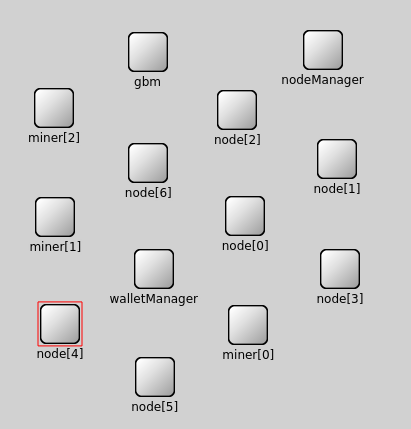
\includegraphics[width=0.5\textwidth]{iblock-qt-network}
	\caption{An \iblock{} network in the OMNeT++'s QT
	environment.}\label{fig:iblock-network}
\end{figure}

Nodes can be of different types, and they can be configured with different
parameters, leveraging the flexibility of the \omnetpp{} framework's
configuration capabilities. In \figref{fig:iblock-network}, two types of nodes
are present: \emph{Miner} nodes and \emph{User} nodes (called just ``node[*]''
in the figure). \emph{Miner} nodes are nodes that contain a \emph{Miner
application} that can mine blocks and earn rewards. \emph{User} nodes are nodes
that have a \emph{TransactionGenerator application} and can send transactions
to the network.

There are other special nodes in the network: The \code{gbm}
(\code{GlobalBlockchainManager}) is responsible of creating the \emph{genesis
block} on startup and removing older blocks from the memory when they are no
longer needed; \code{walletManager} is a node that can be contacted by other
nodes in order to get the address of other nodes' wallets; The
\code{nodeManager} module is used as a directory of all nodes in the network.
Nodes ask the \code{nodeManager} for a reference to another node in the network
when they need to send a message to it. These special nodes will be described
in detail in \secref{sec:impl-global}.

As said before, there are no links between nodes in the network. Instead, nodes
communicate using direct messages sent using the \code{sendDirect()} function
of the \omnetpp{}'s simulation library. Communication between nodes and the
special global nodes is instead done using \emph{Direct Method Calls} (DMCs),
which are an efficient way of calling a method of another module directly,
without the need to send a message.

The choice of using direct messages instead of links was made in order to allow
a fairer comparison of \iblock{}'s performance with other blockchain
simulators, especially with BlockSim \cite{blocksim}, which does not simulate
links between nodes. This choice also simplifies the development of the first
version of the simulator leaving the implementation of a more detailed network
layer for future work.

Each node in the network is a \emph{compound module}. Its internals will be
described in the following sections.
